\begin{question}
\noindent Triangle $T$ has vertices $A(-5,1)$, $B(-3,1)$ and $C(-5,4)$.

\noindent Triangle $T$ is first translated by the vector $\begin{pmatrix} 6 \\ -3 \end{pmatrix}$ to give triangle $U$.

\noindent Triangle $U$ is then reflected in the line $y = 1$ to give triangle $V$.

\begin{center}
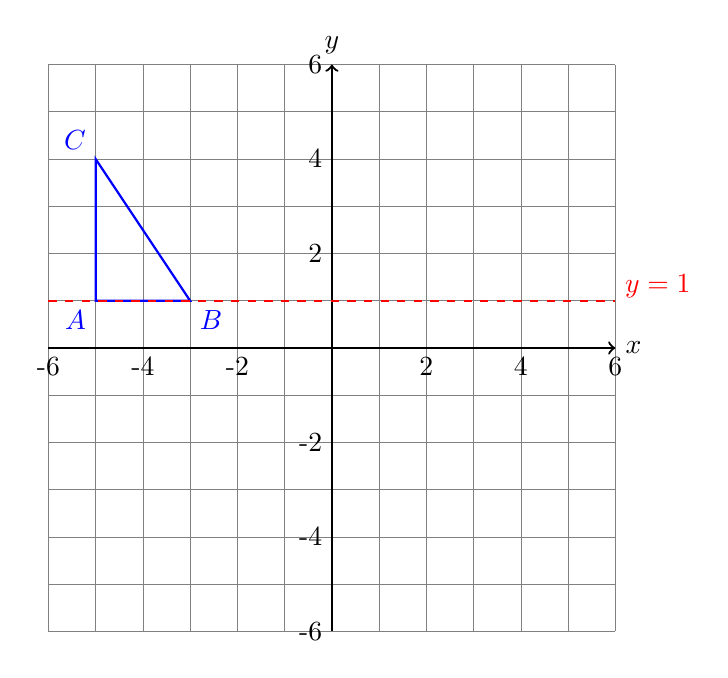
\begin{tikzpicture}[scale=0.6]
    \draw[step=1cm, gray, very thin] (-6,-6) grid (6,6);
    \draw[thick, ->] (-6,0) -- (6,0) node[right]{$x$};
    \draw[thick, ->] (0,-6) -- (0,6) node[above]{$y$};

    \foreach \x in {-6,-4,-2,2,4,6} \node[below] at (\x,0) {\x};
    \foreach \y in {-6,-4,-2,2,4,6} \node[left] at (0,\y) {\y};

    % Triangle T
    \draw[thick, blue] (-5,1) -- (-3,1) -- (-5,4) -- cycle;
    \node[blue, below left] at (-5,1) {$A$};
    \node[blue, below right] at (-3,1) {$B$};
    \node[blue, above left] at (-5,4) {$C$};

    % line y = 1 for reference
    \draw[thick, dashed, red] (-6,1) -- (6,1);
    \node[red, right] at (6,1.3) {$y=1$};
\end{tikzpicture}
\end{center}

\begin{enumerate}
    \item[(a)] On the grid, draw and label triangle $U$, the image of triangle $T$ after the translation.

    \vspace{5cm}
    \answerplain{2}

    \item[(b)] On the grid, draw and label triangle $V$, the image of triangle $U$ after the reflection.

    \vspace{5cm}
    \answerplain{2}
\end{enumerate}
\end{question}
